\documentclass[12pt,a4paper,ngerman]{article}
\usepackage[german,ngerman]{babel} % sorgt dafür, dass "Inhaltsverzeichnis" auf deutsch angezeigt wird, und wahrscheinlich noch ein paar andere Sachen auch


% alles bezüglich Matheformeln

% Gleichungen linksbündig
\usepackage[fleqn]{amsmath}

% wieweit Gleichungen vom linken Rand aus abgerückt werden
\setlength\mathindent{20pt}

\usepackage{amsmath}
\usepackage{amsfonts}
\usepackage{amssymb}

% Schriftart ohne Serifen für Formeln
\usepackage{cmbright}
\SetSymbolFont{largesymbols}{normal}{OMX}{iwona}{m}{n}

\usepackage{mathtools}


% Seitenlayout (Ränder)
\usepackage[top=2.5cm, bottom=2.5cm, outer=4cm, inner=2.5cm, heightrounded, marginparwidth=2.5cm, marginparsep=0.5cm]{geometry}

% Bildunterschriftdesign
\usepackage[font=small,labelfont=bf]{caption}
\usepackage{caption}



\usepackage{graphicx}



% Benutzerdefinierte Farben
\usepackage{color}
\definecolor{light-gray}{gray}{0.95}






% Schriftart für SourceCodeListings
%\usepackage{sourcecodepro}

% Programmcode Formatierung
\usepackage{listings}
\lstset{
	backgroundcolor=\color{light-gray},
	breaklines=true,
	captionpos=b,
	frame=none, % zB leftline oder single
	keepspaces=true,
	keywordstyle=\color{olive},
	%numbers=left,
	numbersep=5pt,
	tabsize=4,
	%numberstyle=\tiny,
    basicstyle=\footnotesize %\ttyfamily
}

% Kopf- und Fußzeile
\usepackage[headsepline,footsepline]{scrpage2}
\pagestyle{scrheadings}
\clearscrheadfoot

% Kopfzeile
%\ihead{Hochschule München - Segway}
\ohead{\headmark}
\automark[subsection]{section}

%Fuߟzeile
\ifoot{\autoren}
\ofoot{\pagemark}


% hiermit kann man später angeben, wer welche Seite geschrieben hat
\newcommand{\autoren}{}
















\usepackage{wrapfig, ragged2e}

\usepackage{float}
\usepackage{fontspec,xunicode}  % dadurch kann man auch äöü direkt im text eingeben



\usepackage[utf8]{inputenc}



% sollte eigentlich Gleichungen linksbündig ausrichten
%\def\changemargin#1#2{\list{}{\rightmargin#2\leftmargin#1}\item[]}
%\let\endchangemargin=\endlist

%\newfontfamily\codefont[]{Hack}
%\lstset{basicstyle=\codefont,breaklines=true}

% sorgt dafür, dass nicht so viel Platz über und unter Gleichungen eingefügt wird
\newenvironment{mathezeug}
 {\setlength{\abovedisplayskip}{00pt}\setlength{\belowdisplayskip}{\baselineskip}}%
 %\csname flalign*\endcsname}
 %{\csname endflalign*\endcsname\ignorespacesafterend}


\newcommand\tab[1][1cm]{\hspace*{#1}}

\setmainfont{Arial}

%\usepackage{mathpazo}
%\setmainfont{Palatino}

\setcounter{secnumdepth}{4} % erlaubt Unter-Unter-Kapitel

% folgendes macht automatisch Links im Inhaltsverzeichnis des Pdfs, die direkt zum Unterkapitel führen
\usepackage[colorlinks,pdfpagelabels,pdfstartview = FitH,bookmarksopen = true,
bookmarksnumbered = true,linkcolor = black,plainpages = false,hypertexnames = false,
citecolor = black] {hyperref}


% für Zitate
\usepackage[style=numeric, backend=bibtex]{biblatex}
\addbibresource{Quellenverzeichnis}  % Bibtex-Datei wird schon in der Preambel eingebunden

% Sachen wegen Literaturverzeichnis
\usepackage{url}
\newcommand*\oldurlbreaks{}
\let\oldurlbreaks=\UrlBreaks
\renewcommand{\UrlBreaks}{\oldurlbreaks\do\\}
%\renewcommand{\UrlBreaks}{\oldurlbreaks\do\a\do\b\do\c\do\d\do\e%
%  \do\f\do\g\do\h\do\i\do\j\do\k\do\l\do\m\do\n\do\o\do\p\do\q%
%  \do\r\do\s\do\t\do\u\do\v\do\w\do\x\do\y\do\z\do\?\do\&}
\usepackage{hyperref}


\usepackage[disable]{todonotes}

%\raggedright % verhindert Blocksatz

% Zeilenabstand = 1.5
\usepackage{setspace}
\onehalfspacing









\begin{document}
\setlength{\parindent}{0pt} % kein Einzug bei Absatzanfang
\captionsetup{singlelinecheck=false}
% !TEX root = SegwayDoku.tex

\begin{titlepage}
\thispagestyle{empty}
\newgeometry{left=3cm,bottom=2cm, outer=2cm, top=2cm}
\begin{flushleft}
\begin{Huge}
\textbf{Hochschule München}
\par\medskip
Projektarbeit Wackelroboter
\end{Huge}
\begin{large}
\par\vspace{5cm}
\begin{figure}[h]
\centering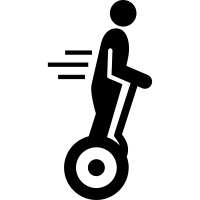
\includegraphics[width=0.3\textwidth]{images/segwayIcon.png}

% würde eine Bildunterschrift erzeugen
%\caption[Eintrag im Abbildungsverzeichnis]{}
\end{figure}

\par\vspace{5cm}

\begin{large}
\begin{tabbing}
Betreuer \hspace{2cm}\= Prof. Dr. Norbert Nitzsche \\\\
Verfasser \> Valentyn Chepil, Stephan Morongowski, \\ \> Severin Schendel, Aleksandar Stoiljkovic, Timo Veit \\
%Adresse \> Hauptstraߟe 45 - 85293 Reichertshausen \\
%Telefon \> 0176-23837636 \\
Fachbereich \> Maschinenbau - MBB \\
Abgabetermin \> 28.2.2018

\end{tabbing}
\end{large}




\end{large}
\end{flushleft}


%\centering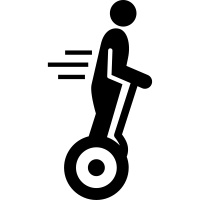
\includegraphics{images/segwayIcon.jpg}
\vfill % Fill the rest of the page with whitespace
\end{titlepage}
\restoregeometry




%\pdfbookmark[1]{Inhaltsverzeichnis}{toc}

% verhindert die Fuߟzeile für die aktuelle Seite
\thispagestyle{empty}

\tableofcontents
\newpage
\thispagestyle{empty}
\listoffigures
\newpage
\setcounter{page}{1}


% hier werden alle Extradateien eingebunden
% !TEX root = SegwayDoku.tex
\renewcommand{\autoren}{Stephan Morongowski}
\newpage
\section{Definition eines roboterfesten Koordinatensystems}

\begin{figure}[h]  % [h] bedeutet, dass das Bild genau an dieser Stelle im Text erscheint
\centering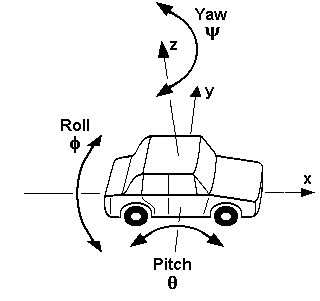
\includegraphics[width=0.6\textwidth]{images/FahrzeugKSys_mod.png}
\caption[Roboterkoordinatensystem]{Roboterkoordinatensystem \newline (Quelle: \cite{roboterKS_Bild})}
\label{robotKSys}
\end{figure}

Zur einheitlichen Bezeichnung wurde das roboterfeste Koordinatensystem (im Folgenden mit KS bezeichnet) wie in Abbildung \ref{robotKSys} zu sehen, ähnlich ISO 88551 festgelegt. Entgegen der häufig anzutreffenden Bezeichnungen der Winkel um die jeweiligen Koordinatenachsen werden im Folgenden die Winkel um
\begin{itemize}
    \item die x-Achse mit \(\alpha\)
    \item die y-Achse mit \(\beta\)
    \item die z-Achse mit \(\gamma\)
\end{itemize}
bezeichnet. \\
Der Ursprung des KS liegt auf der Radachse mittig zwischen den beiden Rädern.\\
Das KS ist ein rechtshändiges KS.\\\\
Die Verdrehung der jeweiligen Räder wird mit \(\varphi_l\) bzw. \(\varphi_r\) bezeichnet. Dabei bezeichnet \(l\) das in positive x-Richtung blickend links liegende Rad und \(r\) das in positive x-Richtung blickend rechts liegende Rad.

\newpage

% !TEX root = SegwayDoku.tex
\renewcommand{\autoren}{Stephan Morongowski}
\newpage
\section{Navigation}
\subsection{Sensorik}
Zur Verfügung stehen folgende Sensoren:
\begin{itemize}
\item Gyros in allen drei Raumachsen
\item Beschleunigungssensoren in allen drei Raumachsen
\item Inkrementalgeber der Räder
\item Ultraschallsensoren
\end{itemize}

\subsection{Bestimmung der Position im Welt-KS}

\subsubsection{Drehung um den Momentanpol}
\label{turningVelocityPole}
Zur Bestimmung der Position des Roboters in einem festen Koordinatensystem können die Inkrementalgeber der Antriebsmotoren benutzt werden.

\begin{figure}[h]  % [h] bedeutet, dass das Bild genau an dieser Stelle im Text erscheint
\centering\includegraphics[width=0.8\textwidth]{images/Kurvenkinematic.eps}
\caption{Rotation um den Momentanpol \newline (Quelle: eigene Darstellung, SM)}
\label{kurvenkinematik}
\end{figure}

Zur Ermittlung der aktuellen Position ist in Abbildung \ref{kurvenkinematik} die Kinematik einer Kurvenfahrt dargestellt, betrachtet für einen gedanklich sehr kleinen Zeitabschnitt. In diesem wird angenommen, dass die Geschwindigkeiten \(v_1\) und \(v_2\) beider Räder konstant bleiben. Dies sorgt für die Vereinfachung, dass der Roboter sich auf einer Kreisbahn um einen für die betrachtete Zeitspanne konstanten Momentanpol bewegt. Im Folgenden sind die durch den Inkrementalgeber erfassten Bogenlängen mit arc bezeichnet.
Es gilt:
\begin{flalign}
    % durch das & Zeichen werden alle Gleichungen an diesem Punkt ausgerichtet
	arc_{Rl} &  = \Delta\gamma\cdot r_{Rl}
	\label{eq:bogenmaß_1} \\
	arc_{Rr} & = \Delta\gamma\cdot r_{Rr}
	\label{eq:bogenmaß_2} \\
	r_{Rr} & = r_{Rl}  + l_a
	\label{eq:achsZuMomentanpol} \\
	\Delta arcs & = arc_{Rr} - arc_{Rl}
	\label{eq:arcsDef} \\
    r_S & = r_{Rr} - \frac{1}{2} l_a
	\label{eq:r_s}
\end{flalign}

Aus \eqref{eq:bogenmaß_1}, \eqref{eq:bogenmaß_2}, \eqref{eq:achsZuMomentanpol}, \eqref{eq:arcsDef} und \eqref{eq:r_s} folgen:
% hier keine Leerzeile machen, sonst wird der Abstand ganz groß
\begin{flalign}
    \Delta\gamma & = \frac{\Delta arcs}{l_a}
	\label{eq:deltaPhi} \\
    r_S & = \frac{arc_{Rr}}{\Delta\gamma} - \frac{1}{2} l_a =
    l_a\left(\frac{arc_{Rr}}{\Delta arcs}-\frac{1}{2}\right)
\end{flalign}

Timo Veit:
Die Verschiebungen aus den Geschwindigkeiten nenne ich erstmal $x_*$.
%In Simulink verwende ich erstmal die Geschwindigkeiten und integriere dann danach, um auf die richtige Einheit zu kommen. Da aus Geschwindigkeit mal Zeit wieder Strecke wird funktioniert das auch.

\begin{flalign}
	x_S &= \frac{x_2-x_1}{2}+x_1	\\
	r_S &=  \frac{l_a}{ \frac{x_2}{x_1}-1} +  \frac{l_a}{2}\\
	\Delta\gamma &= atan( \frac{x_S}{r_S})	
\end{flalign}
Durch Aufsummieren von \(\Delta\gamma\) nach jeder Auswertung der Inkrementalgeber kann somit ein ungefährer Absolutwinkel der Roboterachse zu einem festen KS berechnet werden.
\par\bigskip
Zur Bestimmung des Schwerpunktes in xy-Koordinaten wird die Verschiebung von
\(S_0\) zu \(S_1\) mit trigonometrischen Funktionen berechnet und anschließend aufsummiert. Es gilt:
\begin{flalign}
	\vec{S_1} = \vec{S_0} +
        \begin{pmatrix}
            -\sin{(\Delta \gamma)} \cdot r_S \cdot \sin{(\gamma_0)}
            - (r_S - \cos{(\Delta \gamma)} \cdot r_S) \cdot \cos{(\gamma_0}) \\
            \sin{(\Delta \gamma)} \cdot r_S \cdot \cos{(\gamma_0)}
            - (r_S - \cos{(\Delta \gamma)} \cdot r_S) \cdot \sin{(\gamma_0})
        \end{pmatrix}
	\label{eq:S_1}
\end{flalign}

bzw. vereinfacht:
\begin{flalign}
	\vec{S_1} = \vec{S_0} +
        \begin{pmatrix}
            r_S [\cos{(\gamma_0 + \Delta\gamma)} - \cos{\gamma_0}]  \\
            r_S [\sin{(\gamma_0 + \Delta\gamma)} - \sin{\gamma_0}]
        \end{pmatrix}
	\label{eq:S_1_easy}
\end{flalign}

\subsubsection{Vereinfachung}
\label{easyDeadReckoning}
Nachteilig an der in \ref{turningVelocityPole} beschriebenen Methode sind folgende zwei Punkte: Zum Einen muss eine Geradeausfahrt des Roboters als Spezialfall behandelt werden, da sonst eine Division durch Null erfolgen würde. Zum Zweiten finden die Berechnungen immer nahe einer Singularität statt. Für eine annähernde Geradeausfahrt wird $r_S$ sehr groß und $\Delta \gamma$ sehr klein, was zu großen Berechnungsfehlern führen kann.

Reagiert man nun auf jedes Pulssignal der Inkrementalgeber, wird eine der beiden Größen $arc_{Ri}$ zu Null und der Momentanpol liegt auf diesem Rad, welches sich annähernd nicht bewegt hat. So müssen nur vier Fälle bei der Summation der Lageänderungen beachtet werden:

\begin{itemize}
\item $R_l$ dreht sich vorwärts oder rückwärts
\item $R_r$ dreht sich vorwärts oder rückwärts
\end{itemize}

Für jeden dieser Fälle können nun die Positionsänderungen $\Delta\gamma$, $\Delta x$, $\Delta y$ im roboterfesten KS vorberechnet werden.
\begin{flalign}
    arc_{Rn} & = \frac{2\pi\cdot r_R}{n_{Enc}}  \\
	\Delta\gamma & = \frac{arc_{Rn}}{l_a}  \\
	\Delta x & = \frac{1}{2}l_a\sin{(\Delta\gamma)}  \\
	\Delta y & = \frac{1}{2}l_a ( \cos{(\Delta\gamma)} - 1) 
\end{flalign}
mit der Anzahl der Encoderimpulse pro Umdrehung $n_{Enc}$  \\ und dem Radius der Räder $r_R$. \\ \\
Bei jedem Impuls der Encoder werden nun in Abhängigkeit von $\gamma_0$ die vorberechneten Positionsänderungen mit Hilfe einer Drehmatrix in das Welt-KS transformiert und zu $S_0$ hinzuaddiert. Zu $\gamma_0$ wird jedes Mal nur der konstante Wert $\Delta\gamma$ addiert.
\begin{flalign}
    \prescript{0}{}{S_1} &= \prescript{0}{}{S_0} + \prescript{0}{}{T}_1  \prescript{1}{}{\vec{\Delta s}}
    = \prescript{0}{}{S_0} + 
        \begin{pmatrix}
            \cos{\gamma_0} & -\sin{\gamma_0}  \\
            \sin{\gamma_0} & \cos{\gamma_0}
        \end{pmatrix}
        \begin{pmatrix}
            \Delta x  \\
            \Delta y  
        \end{pmatrix} \\
    \gamma_1 &= \gamma_0 + \Delta\gamma
\end{flalign}

\subsubsection{Berücksichtigung des Kippwinkels}
Obiger Algorithmus setzt voraus, dass der Roboter aufrecht steht. Kippt der Roboter um seine y-Achse, werden alleine durch das Kippen die Encoder verdreht, was zu einer berechneten Positionsänderung führt, die gar nicht stattgefunden hat. Um dies zu kompensieren, reichen die Encoder als alleinige Information nicht aus. Da der Roboter einen Sensor zur Bestimmung des Kippwinkels besitzt, kann nun eine laufende Korrektur vorgenommen werden. Dabei ist zu beachten, dass der Fehler durch das Kippen auch von dem aktuellen Winkel $\gamma$ abhängig ist. Kippt der Roboter z.B. bei einem $\gamma$ von $0°$, entsteht ein Fehler in x-Richtung. Würde er sich nun auf der Stelle drehen auf ein $\gamma$ von $90\degree$ und der bei einem $\gamma$ von $0\degree$ entstandene Fehler weiterhin einfach abgezogen, würde die Position nun einen Ort mit einem Fehler in y-Richtung anzeigen. Deshalb wird bei jedem Encoderimpuls die Änderung des Kippwinkels im Vergleich zur letzten Encoderauswertung umgerechnet in einen Weg in x-Richtung des roboterfesten KS, anschließend in das Welt-KS transformiert und gleichzeitig mit der durch in Abschnitt \ref{easyDeadReckoning} falsch berechneten Welt-Position aufsummiert.

\begin{flalign}
    \prescript{0}{}{S_1} &= \prescript{0}{}{S_0} + \prescript{0}{}{T}_1  \prescript{1}{}{\vec{\Delta s}}
    = \prescript{0}{}{S_0} + 
        \begin{pmatrix}
            \cos{\gamma_0} & -\sin{\gamma_0}  \\
            \sin{\gamma_0} & \cos{\gamma_0}
        \end{pmatrix}
        \begin{pmatrix}
            \Delta x  \\
            \Delta y  
        \end{pmatrix} \\
    \gamma_1 &= \gamma_0 + \Delta\gamma
\end{flalign}


\newpage







\renewcommand{\autoren}{}
\newpage
\thispagestyle{empty}
\renewcommand\refname{Literaturverzeichnis}
\printbibliography
\newpage

\appendix
%\thispagestyle{empty}
\renewcommand{\autoren}{Anhang}
\setcounter{page}{1}


\end{document}
